\documentclass[11pt
  , letterpaper
  , article
  , oneside
  %  , twoside
  , showtrims
 % , draft
]{memoir}


\usepackage{docs}
\usepackage[numbers]{natbib}
\usepackage[autostyle]{csquotes}
\usepackage{blindtext}
\usepackage[overload]{textcase}
\setsecnumdepth{subsection}

\UseRawInputEncoding
%\Urlmuskip=0mu plus 1mu

\begin{document}
\docnum{AL-xxxx-xxxx}
\docrev{A}
\docstatus{Working}
\doctype{Note}
\doccategory{AL7000}
%% Date
%%
\date{\today}
%% Document Title
%%
\title{EPICS IOC Reference Guide}
\subtitle{ALS-U Controls Technical Document}
% Document Author(s), if more than one author,
%% use \newline instead of \\ or \linebreak in order to separate them
\author{Sangil Lee}

\showtrimson

\jhleetitle
\newpage
\tableofcontents
\newpage

%\mainmatter


\chapter{Revision History}
\begin{table}[!h]
  \centering
  \begin{tabularx}{\textwidth}{l|r|X}
    \toprule
    \textbf{Rev.} & \textbf{CM number}  & \textbf{Description of Change} \\
    \midrule
    A             &                     & Add reference note for IOC development \\
    \bottomrule
  \end{tabularx}
\end{table}

\chapter{Approvals}
The following individual(s) shall approve this document:
\begin{table}[!h]
  \centering
  \begin{tabularx}{\textwidth}{l|l}
    \toprule
    \textbf{Approver} & \textbf{Project Role} \\
    \midrule
    William Wardon        & Accelerator Electrical Systems Lead  \\
    \midrule
    Carlos Serrano Pareja & Controls and Instrumentation CAM \\
    \midrule
    & \\
    \midrule
    \multicolumn{2}{l}{\tiny Windchill Approved / Concurred By} \\
    \bottomrule
  \end{tabularx}
\end{table}

\chapter{Abbreviations and Acronyms}
\begin{table}[!h]
  \centering
  \begin{tabularx}{\textwidth}{ll}
    ALS   & Advanced Light Source \\
    ALS-U & Advanced Light Source Upgrade \\
    LBNL  & Lawrence Berkeley National Laboratory \\
    N/A   & Non Applicable \\
    EPICS & The Experimental Physics and Industrial Control System \\
    IOC   & Input-output controller
  \end{tabularx}
\end{table}
\chapter{Introduction}

\section{Scope}
\begin{itemize}
\item The purpose of this document is to organize the references necessary for EPICS IOC development.
\item This document attempts to be a simple guideline, not to be a mandatory procedure.
\item This document is intended to share experiences and considerations with developers based on previous experiences in the EPICS IOC development stage.
\end{itemize}

\section{Target Audience}
This document is targeted to ALS/ALS-U Controls System engineers and technical stakeholders. It is assumed that the target audience has a technical background in the EPICS development, a Unix/Linux environment, and a revision control system, specifically, \texttt{git}. This mainly includes information on emprical activities for EPICS IOC development.

\chapter{Recommend Network Configuration}
The EPICS provides a framework to integrate a lot of distributed control components. The main point of the distributed control system is to config the efficient and flexible network. 

\section{Dividing EPICS Network and Local Network}
Many equipment devices support for UDP/TCP/IP protocol to control them. Therefore, it is good to separate the network for controlling field I/O and the network for EPICS IOC. Figure~\ref{fig:network_configuration} shows that the network configuration is divided into an EPICS network and a local network based on the IOC. EPICS IOC server through two NIC interfaces isolates each other. A network switch connected to the IOC server uses an L2 switch. This can prevent packet looping errors caused by the L3 switch even if the network is incorrectly configured. This configuration also minimizes IP address list management based on IOC.

\newpage
\begin{figure}[!hbt]
	\centering
	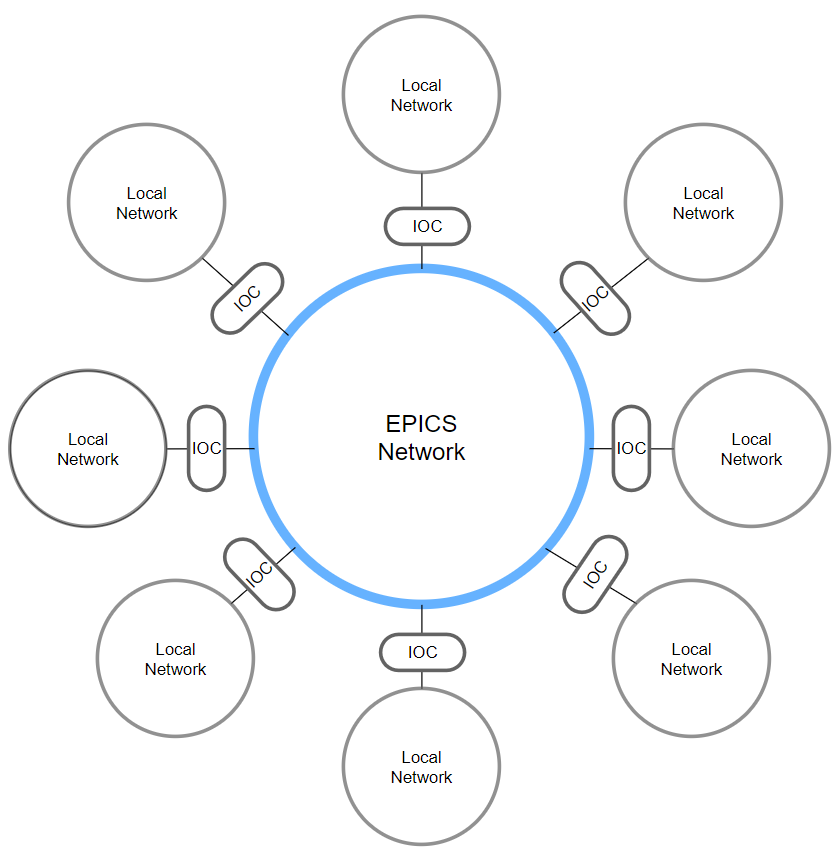
\includegraphics[width=0.8\textwidth]{./pictures/network_conf.eps}
	\caption{
		Dividing Network Configuration by IOC.
	}
	\label{fig:network_configuration}   
\end{figure}

\chapter{Hierarchical Logic-Partitioning}
For the configuration of the integrated control system of large and distributed facility, it is necessary to define the location of the control logic. Figure~\ref{fig:logic_partition_layer} shows three logic configuration with three layers. By setting the position of the appropriate logic partition according to the layer composition, the actual control software operation and configuration management are carried out. The purpose of the logic partition is to clarify the responsibility of implementing the logic according to the location of the logic for distributed control and the SW configuration management for it.

\begin{figure}[!hbt]
	\centering
	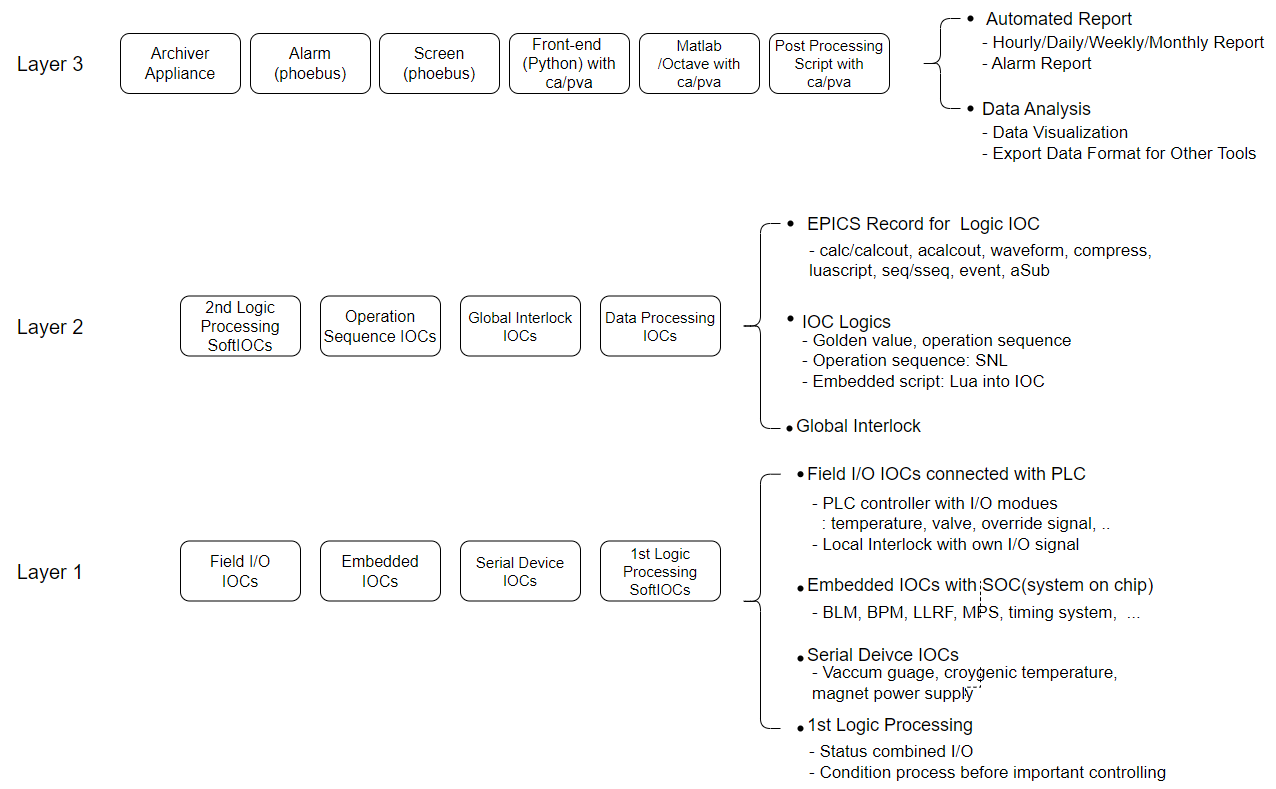
\includegraphics[width=0.99\textwidth]{./pictures/logic_partition_layer.eps}
	\caption{
		Logic Partitioning by Layer 3
	}
	\label{fig:logic_partition_layer}   
\end{figure}
\newpage

\section{Layer1 - EPICS IOC Logic related field I/O}

\subsection{Recommends}
The logic related to field I/O is located in the layer1 configuration of the logical partition. Components of the logic to be located in layer 1 are as listed below.

\begin{itemize}
	\item IOCs connected PLC controllers with field I/O modules
	\item Embedded IOCs
	\item Serial specific IOCs for serial communication device
	\item SoftIOCs for logic extension
\end{itemize}

\newpage
\subsection{Applications }
Table ~\ref{table:logic_layer1} shows the suggested IOC examples for the layer1 configuration.
\begin{table}[!h]
	\centering
	\begin{tabularx}{\textwidth}{l|l|l}
		\toprule
		Field I/O Logic  & Descritption       & Example IOC Logics \\
		\midrule
		PLC controller & Logic on Field I/O Controller		& Field I/O, Interlock, Local PID \\
		SoC controller & \begin{tabular}{@{}l@{}}Embedded IOC between \\CPU core and FPGA cell\end{tabular}
		& \begin{tabular}{@{}l@{}}Timing, MPS, \\LLRF and so on\end{tabular}  \\
		Chassis controller & High sampling DAQ system  
		& \begin{tabular}{@{}l@{}}Beam diagnostics \\(ACCT, DCCT, BLM)\end{tabular}  \\
		Serial controller & Serial device controller    & Vacuum gauge,  Magnet \\
		SoftIOCs extension & Combination logic with local I/O   
		& \begin{tabular}{@{}l@{}}Health status,\\Pre-condition process\end{tabular}  \\
		\bottomrule
	\end{tabularx}
	\caption{Suggestions for Layer1 Logic}
	\label{table:logic_layer1}
\end{table}

The purpose of the layer1 configuration ~~

\section{Layer2 - Middle Layer IOCs}
\subsection{Recommends}
The logic related to configuration of the layer2 extends IOCs based on ethernet for integration of field I/O IOCs. This is to expand in the network at the upper level when it exceeds the scope of local I/O such as global interlock.
Such types of applications can be enumerated as follows:
\begin{itemize}
	\item Global interlock system(by integrating each local interlock signal)
	\item Operation sequencing by system(with SNL)
	\item Such as beam permit system(with combinations for each health states)
	\item Golden value system for each local group
	\item Global alarm system: representative alarm between linked alarms
\end{itemize}

\newpage
\subsection{Applications }
Table ~\ref{table:logic_layer2} shows the suggested IOC examples for the layer2 configuration.
\begin{table}[!h]
	\centering
	\begin{tabularx}{\textwidth}{l|l|l}
		\toprule
		Logics for Layer2  & Descritption       & Example IOC Logics \\
		\midrule
		DB Record IOCs & \begin{tabular}{@{}l@{}}EPICS DB record\\processing with CA \end{tabular}		
		& \begin{tabular}{@{}l@{}l@{}}DB record processing\\(calc/calcout,acalcout,waveform,\\ compress,seq/sseq,event,sub/asub)\end{tabular} \\
		Sequence IOCs & \begin{tabular}{@{}l@{}}Logic combined \\with field I/O logics\end{tabular}
		& \begin{tabular}{@{}l@{}}SNL sequence logic\\with DB processing \end{tabular}  \\
		Global IOCs & \begin{tabular}{@{}l@{}} Logic integrated \\into the higher network \end{tabular}  
		& \begin{tabular}{@{}l@{}}Global alarm/interlock \\(BPS, alarm triggering, postmortem)\end{tabular}  \\
		\bottomrule
    \end{tabularx}
	\caption{Suggestions for Layer2 Logic}
	\label{table:logic_layer2}
\end{table}


\section{Layer3 - Top level application logics }
\subsection{Recommends}
The logic of the layer3 configuration is located at the top. Layer3 logic mainly uses a scripting language that should be executed on the front-end to maximize flexibility.
\newline\newline
Script languages supported by the EPICS interface module are as follows:

\begin{itemize}
	\item Python - Beam dynamics, front-end data analysis/visualization
	\item Matlab / Octave - Beam dynamics
	\item Ruby
	\item Lua
	\item Golang / Rust(another native compiling language)
	\item Shell(Bash, csh, zsh)
\end{itemize}

\newpage
\subsection{Applications }
Table ~\ref{table:logic_layer3} shows the suggested top level service examples for the layer3 configuration.
\begin{table}[!h]
	\centering
	\begin{tabularx}{\textwidth}{l|l|l}
		\toprule
		Top Service  & Descritption       & Example Service \\
		\midrule
		Alarm & Phoebus Alarm, Alarm Report	& \begin{tabular}{@{}l@{}}Alarm(Panel, Tree, Table, History)\\Alarm Procedure(Alarm code) \end{tabular} \\
		Data Archiving & EPICS Data Archive, DAQ Archive
		& \begin{tabular}{@{}l@{}}Archive Appliance(with ca/pva)\\HDF5 file for DAQ \end{tabular}  \\
		Post Processing & Reporting, Data Analysis  
		& \begin{tabular}{@{}l@{}l@{}}Automated Report\\(Hourly, Daily, Weekly, Monthly) \\Visualization for Beam Transmission\end{tabular}  \\
		Beam Dynamics & Beam Parameter Tunning  & On-line model and so on \\
		Golden Value Check& Accelerator Status Verifying   
		& \begin{tabular}{@{}l@{}}Acclerator status,\\Beam Permit, Emergency Process\end{tabular}  \\
		\bottomrule
	\end{tabularx}
	\caption{Suggestions for Layer3 Logic}
	\label{table:logic_layer3}
\end{table}


\chapter{Operation Screen}
In order to integrate and manage the operation screen developed for each group, the entire layout is proposed as shown in Figure~\ref{fig:opi_layout}. The layout is largely composed of header, footer and side panel. Header consists of selection buttons for each operation group. The lateste alarm list is located at the footer. The left side panel. The left side panel displays the initial screen of each sub group according to the group. This side panel can be hide or show. 
\newpage
\begin{figure}[!hbt]
	\centering
	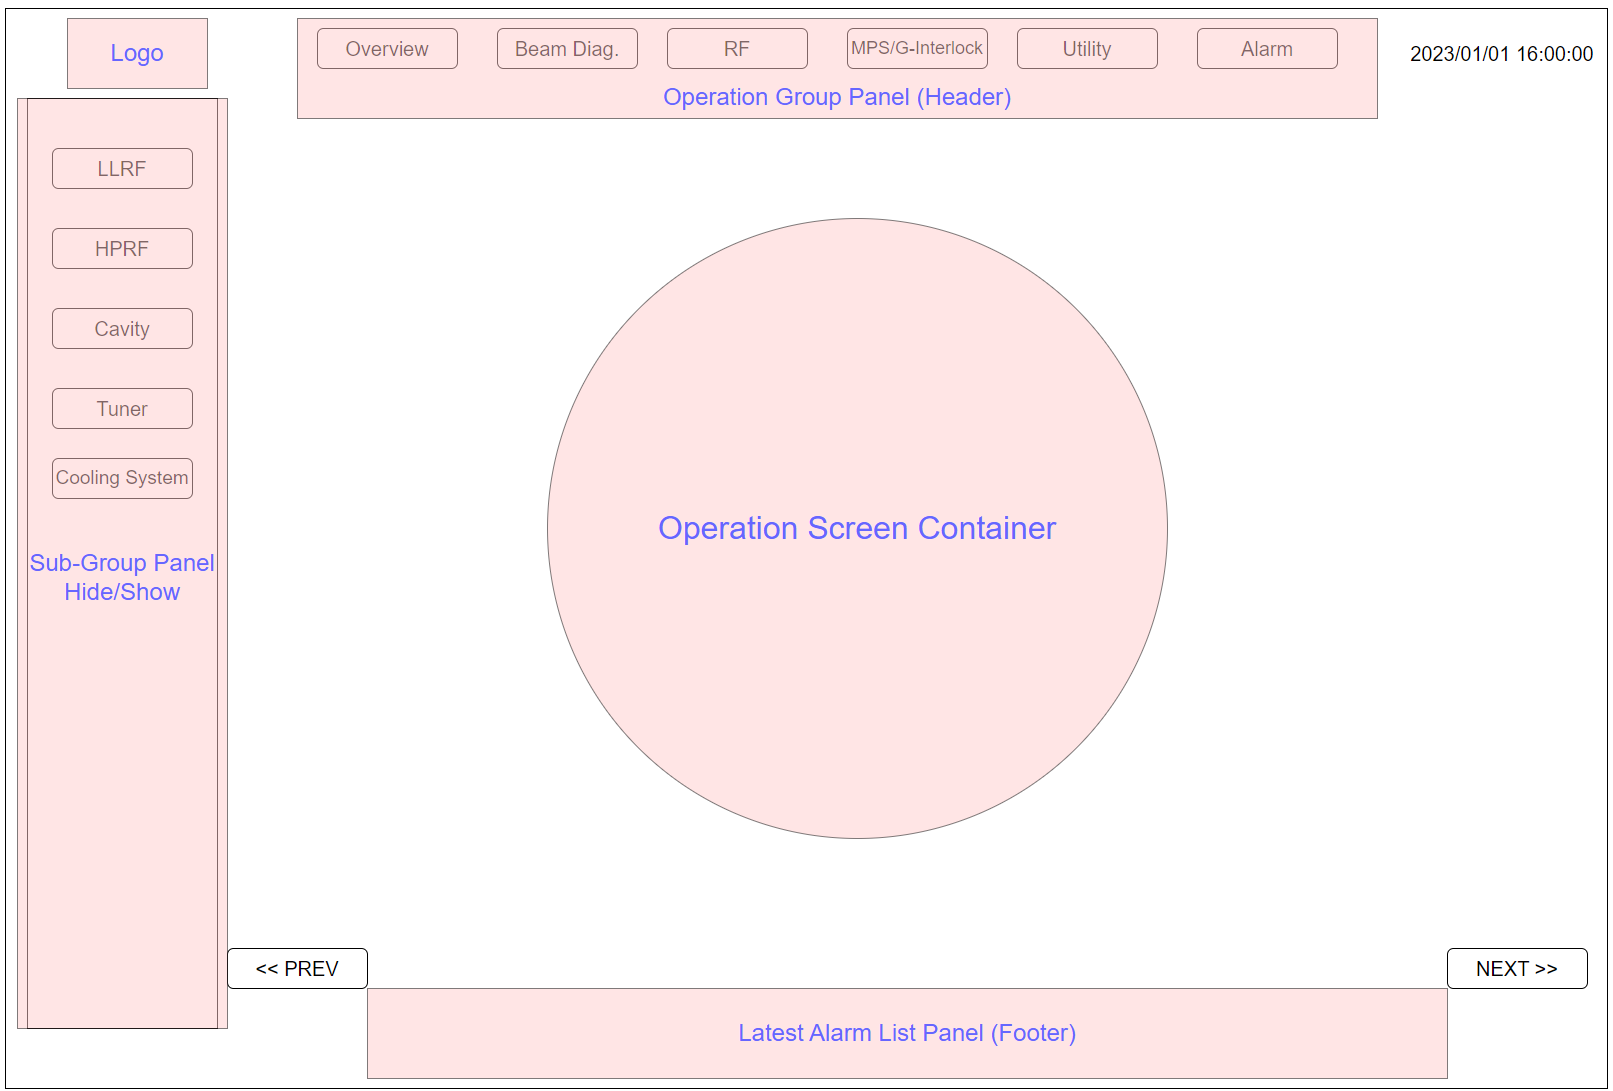
\includegraphics[width=0.8\textwidth]{./pictures/opi_layout.eps}
	\caption{
		Operation Screen Layout
	}
	\label{fig:opi_layout}   
\end{figure}
The center area of the screen is selected as the initial screen of the selected group, and the screen is moved to each screen with navigation buttons connected to each screen.
Here figure~\ref{fig:opi_example} is one of the real example screens. 

\begin{figure}[!hbt]
	\centering
	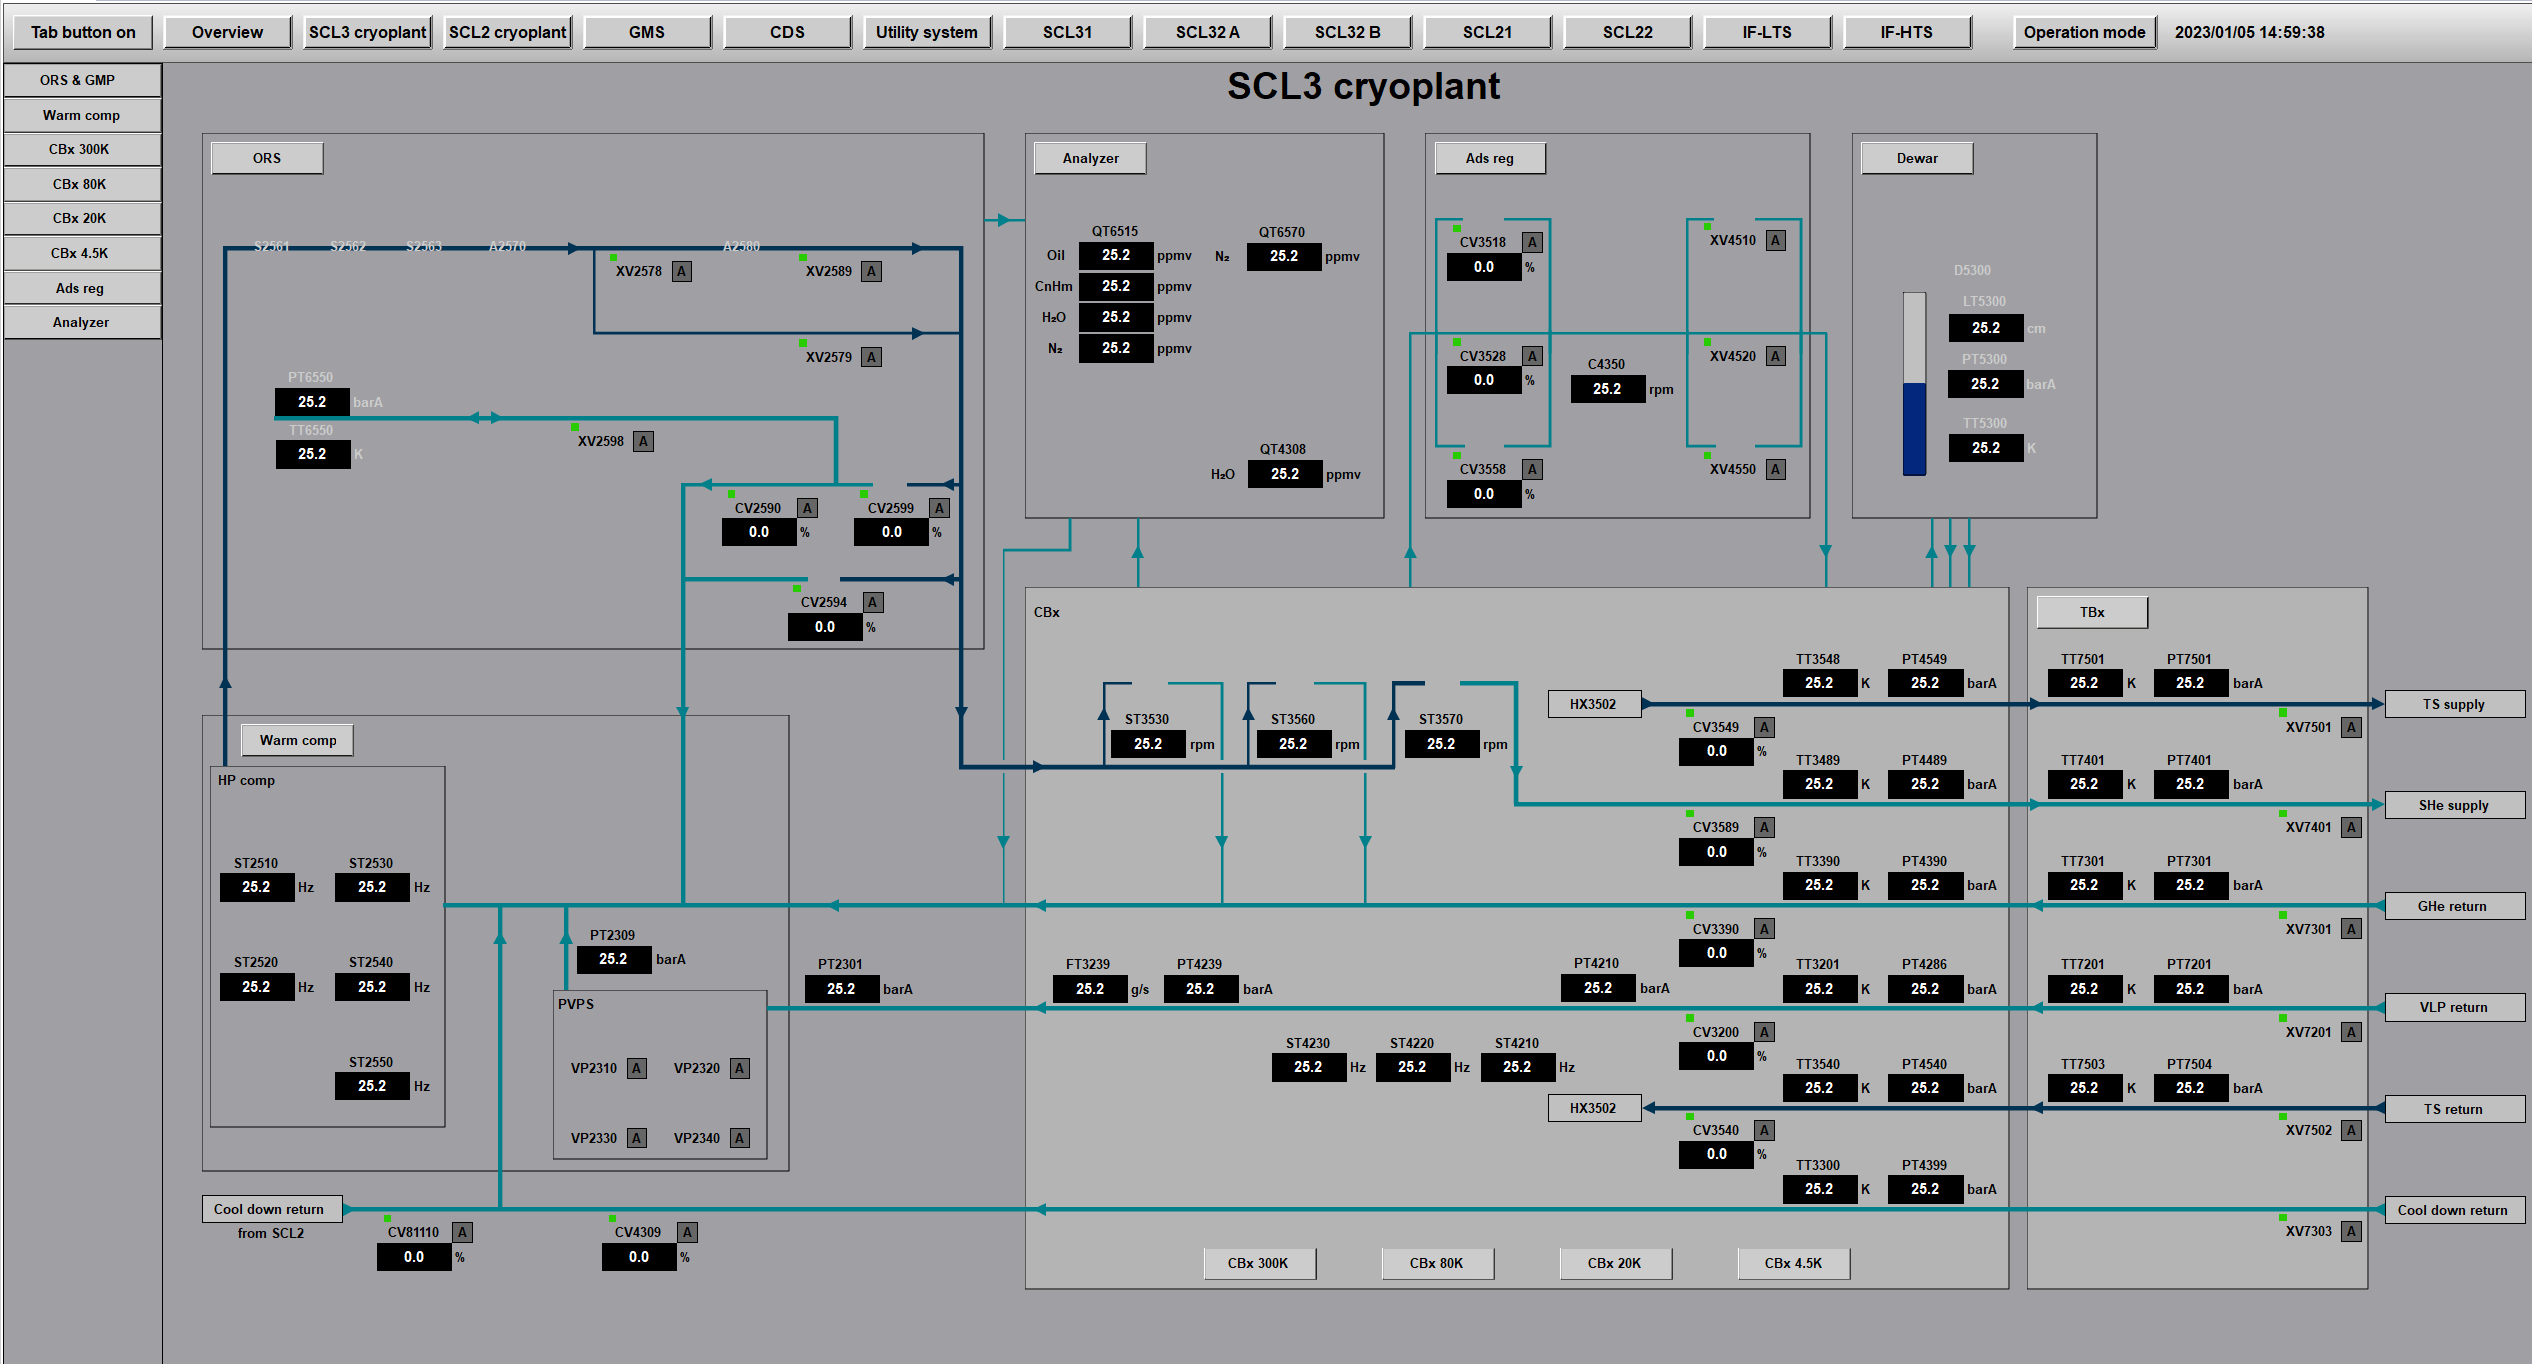
\includegraphics[width=0.8\textwidth]{./pictures/opi_example.eps}
	\caption{
		Operation Screen Example
	}
	\label{fig:opi_example}   
\end{figure}

\newpage
\chapter{Alarm and Interlock}
Considerations for alarm and interlock should be actively reflected in the EPICS IOC development stage. When considering an alarm, it is necessary to define whether it should be linked with interlock when it is out of alarm. 

\section{Definition Scope of Alam/Interlock}
Alarm and interlock are defined based on the following items.

\begin{itemize}
	\item Scope of Alarm/Interlock
	\subitem Local Alarm: alarm related to physical I/O signal
	\subitem Global Alarm: alarm linked between EPICS IOCs logically
	\item Sequence of Alarms/Interlock
	\subitem Single Alarm: defines the case where the physical signal is a single that is not related to each other.
	\subitem Chain of Alarm: the case when the alarm of one physical signal propagates with continuous chain
\end{itemize}

Table~\ref{table:scope_alarm} describes the ranges for alarms or interlock. 

\begin{table}[!h]
	\centering
	\begin{tabularx}{\textwidth}{l|l|l}
		\toprule
		Range of Alarm    				& Descritption       & Example Logics \\
		\midrule
		Local(alarm, interlock)         & Via physical signal  & Temperature, Pressure ... \\
		Global(alarm, interlock)        & Out of scope local area & Global alarm logic between IOCs\\ 
		Sequence of (alarm, interlock)  & Propagation of signal   & Chain of vacuum pressure \\
		Alarm (report, procedure) 	    & Post processing for alarms & Alarm report and procedure \\
		\bottomrule
	\end{tabularx}
	\label{table:scope_alarm}
	\caption{Range of Alarm}
\end{table}

\section{Other Comments of Alam/Interlock}
\begin{itemize}
	\item Comments for alarms:
	\newline
	- Review and respond to the need to change the alarm setpoint value for each signal in each operation mode.
	\newline
	- In some cases, it is more efficient to operate Alarm PV by creating its own Alarm Tag in PLC.
	\newline
	- In the case of an alarm that cannot be ignored, the corresponding alarm event must be prepared an alarm procedure.(Alarm post processing: Alarm procedure/report for alarm event)
		
	\item Comments for interlock
	\newline
	- If it is out of the scope of the alarm, consider linking with the global interlock logic.
	\newline
	- Prepare global interlock logic in addition to the slow interlock system consisting of real physical signals
\end{itemize}

\section{Alarm Configuration - Phoebus Alarm}	
\begin{itemize}
	\item EPICS/IOCs/Phoebus\_Alarm\_Setup\/alarm-server\_setup.sh(kafka/config/zookeeper.properties,
server.properties)
	\item settings.ini(Phoebus)
	\item demonstration for example (alarm\_topics: Accelerator, Demo)
	\item kafka(alarm panel / alarm tree / alarm table)
	\item elasticsearch(alarm log table(alarm history))
	\item generate EPICS demo.db
	\item generate alarm model config file (demo.xml / test.xml)
	\item Hierarchical golden value design for alarm panel
	\subitem Golden alarm value topic configuration
	\subitem Alarm group(Group1 - Group2) into alarm topic
\end{itemize}

\chapter{A few principles for logical partitioning}
The advantage of the EPICS distributed control system is that control logic can be written easily at any location based on a network in a distributed environment. Therefore, it is necessary to accurately identify the location of the corresponding control logic to prevent errors in software configuration management and control logic. 

\section{Scope for Control Logic}
In order to develop a stable control logic, configure the control logic according to the following principles.

\begin{itemize}
	\item Determination of control logic location according to the layer as described above.
	\item Logic partition management
	\newline 
	- Management of the designated person in charge according to the SRS number of the control logic.
	\item Local field logic(PLC, FPGA, Local Controller) with connected field I/O directly, Layer1.
	\newline
	- For example, determining whether to execute the PID logic on the PLC/FPGA or on the IOC(epid record).
	\item Global logic(layer2 or layer3) based on ethernet out of the scope of local field logic.
	\item Management of conflicts with the logic of each distributed environment.
	\item Control logic of serial devices should be avoided in the PLC. Much better control in EPICS IOCs directly.
	\item Scalable server operation to reduce downtime for control logic modifications.
	\item EPICS DB Records suitable for extending control logic: sub/aSub, calc/calcout, compress/waveform, scalcout/acalcout, luascript, seq/sseq
\end{itemize}

\section{Override Function for Malfunction, Invalid Sensor }
In the case of sensors related to major interlocks and alarms, it is difficult to operate due to the continuous alarm logic or interlock logic due to the Invalid state of the sensor. In this case, the function of overriding the actual physical signal value to a value within the normal range by the operator is a very necessary element to increase the efficiency of accelerator operation.

\begin{itemize}
	\item Invalid sensor(aging, disconnected signal line)
	\item When the sensor signal needs calibration.
	\item Operation of interlock logic by invalid sensor signal
\end{itemize}
The override function can reduce downtime for system operation.

\chapter{Recommends for Optimized IOC}
This section describes some helpful tips for EPICS IOC development.


\section{Protecting for Human Factor Error}
Human factor error is the most common problem for system error. To prevent this error, several items are suggested from the IOC design point of view.

\begin{itemize}
	\item Appropriate using of each output record's DISP field(Disable putField, in dbCommon.dbd)
	\newline
	- In the case of actual physical signals such as triggers, they shou ld not be triggered before setting the DAQ parameters. In this case, if the DISP field of the trigger PV is set to true, the operation value is not reflected.
	\item Using seq/sseq record for continuous parameter settings
	\newline
	- When necessary to define the precedence of setting parameters
	\item HOPR/LOPR field of analog output record
	\newline
	- Can be set valid range for the analog output record, if a value in an invalid range is entered, it is ignored.
	\item Much better multiple EPICS sequences(PROD\_HOST) than one complex sequence logic for operation.
	\newline
	- Useful to develope the incomplete logic without downtime for IOC different logic process in the commissioing phase.
\end{itemize}

\section{DB Record Processing}
In addition to the general use of EPICS DB, it will be look into the matters to be considered from the system design point of view.

\begin{itemize}
	\item Using of PROC(Processing) field(SCAN=”Passive”) in the sequencer
	\newline
	- user-defined processing time, optimized db processing and network resource
	\item Using seq/sseq record for continuous parameter settings
	\newline
	- 
	\item Redefining src/menuScan.dbd
	\newline
	- Create scan thread defined by user.
	\newline
	- When need the faster scan time for DAQ.(menuScan\_05\_second, ".05 second")
	\newline
	- When need the slower scan time verifying H/W lifecycle time.(menuScan3600\_second, "1 hour")
	\newline
	- Useful to make flexible EPICS IOCs.
	\newline
	- Good to make periodic alarm(hourly, daily, weekly, monthly)
	\newline
	- Optimum processing time for saving cpu resources
\end{itemize}

\section{OPI Rules or Scripts for Control Logic}
Sometimes OPI rules or scripts are used when setting various types of control setting parameters. In this case, configuration management for sw logic is required for each OPI and confusion about logic location occurs. Therefore, the basic principles for when OPI rules and scripts must be used are defined as follows.

\begin{itemize}
	\item The case that should be given dynamic movement to a graphic object.(widget position, blinking, gradient, ...)
	\item The case applying the navigation function of the operation screen. (visualization for beam analysis)
	\item If you need to apply the set values of several parameters sequentially, use seq/sseq/luascript record of IOC instead of developing with rules or embedded scripts.
\end{itemize}

\section{Macro Rule}
Clarify the rules for using Macro for PVName used in IOC, cs-studio or Phoebus. This is to prevent errors about pv-naming between users and developers due to confusion about the use of delimiters used between macros. The items below are basic recommendations. In ALS/ALS-U, it is assumed that "\$(P)" and "\$(R)" are used for the PV naming macro.

\begin{itemize}
	\item Do not use delimiter between macros. 
	\newline
	For instance, "\$(P)-\$(R):Signal" or "\$(P):\$(R):Signal"
	\item Attach delimiter at "\$(R)" macro
	\newline
	For instance, "\$(P)\$(R)Signal" in IOC or Phoebus
	\newline
	Macro instance, "P=A, R=-B:", Final PV name: "A-B:Signal"
\end{itemize}

A good macro convention maximizes reproducibility in the development of IOCs and process screens.

\chapter{Accelerator Optimization Operation}
For the optimized operation of the accelerator, it is designed by dividing it into three areas.

\begin{itemize}
	\item Verification of accelerator health status.
	\item Optimized accelerator operation.
	\item Predictable status for accelerator operation.
\end{itemize}

\section{System Readiness via Golden Value}
Find the representative "Golden Value" from each operating system and verify the system readiness.

\begin{itemize}
	\item Device state monitoring(Field controller status, EPICS IOC readiness)
	\newline
	- Memory/CPU load of AVG(5min), Heartbeat, Sub-instruments and so on.
	\item Own network packet information(Inbout/Outbound)
	\item Health status for sub-components connected.
	\item Hardware lifecycle information(epicsTimestamp) for hardware replacement cycle monitoring
	\item Alarm system through golden value for each system.(Local alarm, Group alarm, Sequence alarm)
\end{itemize}

\section{Algorithm to Find Golden Value/Optimum Value}
Apply the necessary algorithm to find the golden value or optimum value for each system.

\begin{itemize}
	\item Linear/Polynomial Waveform Regression.
	\newline
	- Real-time data analysis through regression algorithm by collecting atomic values of the same layer into a waveform
	\item Kalman filter.
	\newline
	- Accuracy improvement by using SW algorithm for sensor's hardware resolution.
	\item Frequency Domain Analysis(FFTWaveform, Fast Fourier Transformer).
	\newline
	- Using vibration/pressure sensor, analysis frequency from pressure signal source.
\end{itemize}

\section{Automated Procedure}
By using alarm triggering from alarm system, it can be performed the automated procedure. Figure~\ref{fig:auto_procedure} shows the flow of executing procedures for various alarm events. It can generate reports such as hourly, daily, weekly and monthly by utilizing event record and 1 hour scan.

\begin{figure}[!hbt]
	\centering
	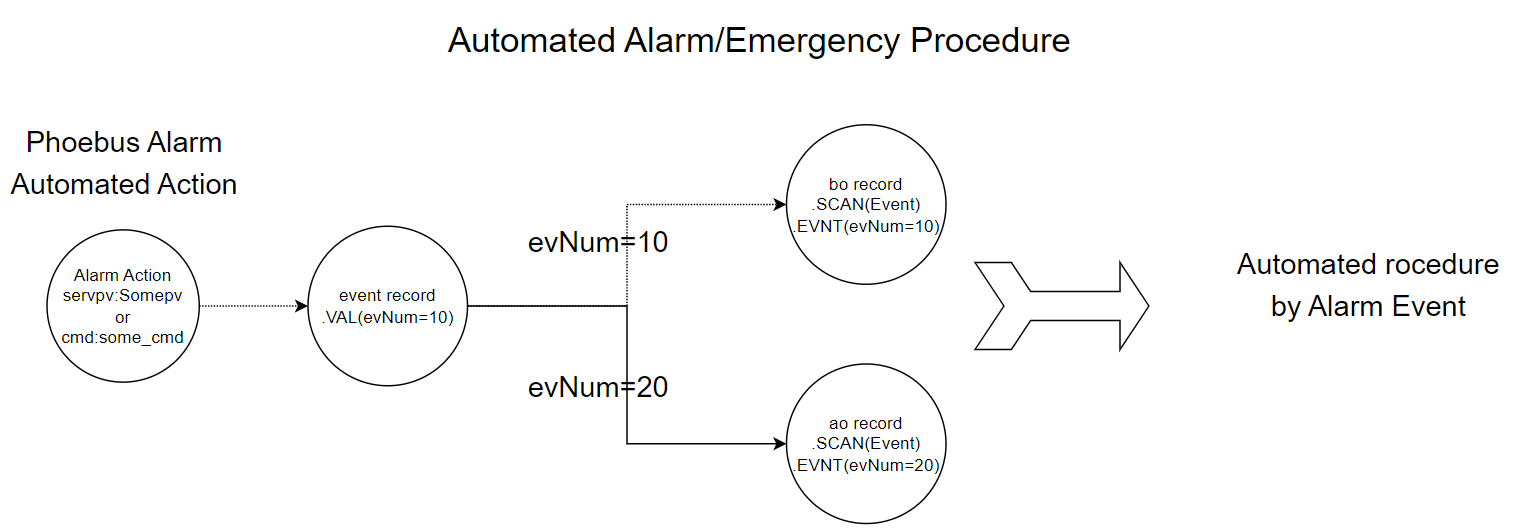
\includegraphics[width=0.99\textwidth]{./pictures/auto_procedure.eps}
	\caption{
		Automated Alarm/Emergency Procedure by Alarm Event
	}
	\label{fig:auto_procedure}   
\end{figure}

\newpage
\appendix
\newpage
\chapter{Make Base Application: manual procedure}
\renewcommand{\thechapter}{A}

\backmatter
%\bibliographystyle{unsrt}
%\bibliographystyle{plainnat}
%\bibliographystyle{abbrvnat}
\bibliographystyle{unsrtnat}
%\bibliographystyle{chicago}
\bibliography{./refs}


\end{document}
